\documentclass[main.tex]{subfiles}
\setlength{\columnsep}{3cm}
\begin{document}

\addtolength{\tabcolsep}{-2pt}

% covered in this section:
% - speedup
% - Amdahl, Gustafson
% do not cover task granularity. talk about this one chapter later maybe, before fork/join and so on. next chapter would be about dividing tasks in Java.
\section{Measuring Parallelism}
In this chapter, we are thinking about parallel programs again. But, instead of concering us with implementing actual programs, we are going to think very abstractly about them. We care about measuring their parallelism and in particular how programs scale with using more processors.

\subsection{Performance} \label{Performance}
\subsubsection{Speedup} \label{Speedup}
Before we take a look at different ways of measuring performance, we first need to introduce some terminology. To that end, let $P$ denote the number of processors available during the execution of a program.
\begin{definition}
$\mathbf{T_P}$ is the time it takes the program to execute on $P$ processors.
\begin{remark}
$T_\infty$ denotes the execution time when we have as many processors at our disposal as is required to get the best-possible execution time.
\end{remark}
\end{definition}
We will usually use $T_1$ to talk about the \textit{sequential} and $T_\infty$ to talk about the \textit{minimum} execution time of a program. When talking about performance in general, we will use $T_P$.
\begin{definition}
The \textbf{speedup} of a program is
\begin{equation*}
    S_P := \frac{T_1}{T_P}
\end{equation*}
\end{definition}
The speedup is essentially the ratio of the sequential execution time to the execution time given $P$ processors.\\
Naively, we might expect the speedup of our program to always be $S_P = P$, i.e. $T_P = T_1 / P$. This would mean perfect linear speedup. However, in reality we usually see \textit{sub-linear} speedup, caused by additional overheads due to inter-thread dependencies, thread creation, thread communication and memory-hierarchy issues.

%==============================================================================================================================

\subsubsection{Amdahl's Law} \label{Amdahl's Law}
Gene Amdahl was an American computer scientist. In 1967, he published a paper titled \textit{Validity of the Single Processor Approach to Achieving Large Scale Computing Capabilities} that coined \textit{Amdahl's Law}. In the paper, Amdahl was defending single-core processors. As an influential figure, Amdahl's paper had significant impact on the industry and strengthened the position of the single-core processor against upcoming multi-core systems. The argument of Amdahl is simple: Given any program, it has some fraction that is sequential (cannot be parallelized). So, even given a machine with lots of processors, the best that can be achieved is to decrease the time required for the \textit{parallelizable} part of the program. Adding more processors cannot possibly do anything about the purely sequential part of the program. So, even if we have a program that is 90\% parallelizable, we cannot get below 10\% of its runtime by parallelizing, even with an infinite number of processors. This means that in order to make great improvements in computing speed, the focus should lie on improving the sequential performance of computers instead of focussing on building multi-core systems.\\
The assumption of Amdahl's law is that the work is fixed. We can visualize the work partitioning on the processors Amdahl's law assumes:

\begin{figure}[H]
    \centering
    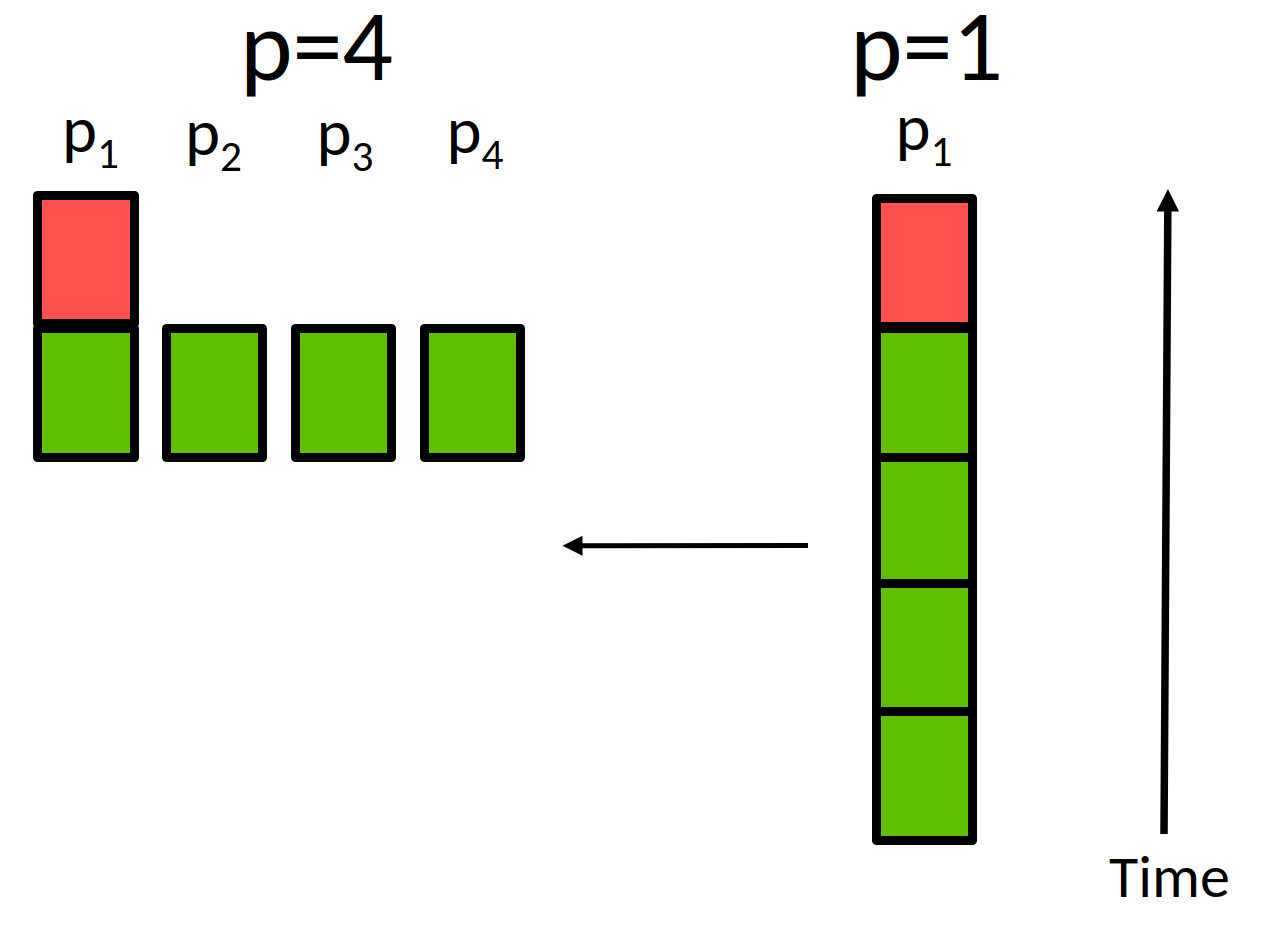
\includegraphics[scale=0.15]{amdahl.png}
    \caption{Red Part is Sequential Work, Green Part is Parallelizable Work.}
\end{figure}

\noindent When we have \textbf{P} processors, each processor has to execute \(\frac{1}{P}\) of the parallelizable part. One processor additionally has to execute the entire serial part. This one processor becomes the bottleneck and we consider the runtime on \textbf{P} processors to be the runtime of this one processor (because the others can execute their part in parallel to it and thus do not prolong the runtime).

Let $W_{ser}$ denote the time spent doing non-parallelizable, serial work and $W_{par}$ denote the time spent doing parallelizable work.\\
We then write:
\begin{equation*}
    T_1 = W_{ser} + W_{par}
\end{equation*}
In above figure, $W_{ser}$ is the red part and $W_{par}$ is the four green parts stacked on top of each other. Thus, $T_{1}$ is the sum, which amounts to the sequential execution time of the entire progam. Let us now derive Amdahl's law:\\[3mm]
$W_{ser}$ remains constant as we increase the number of processors, since the program we execute is fixed (and we assume no multi-processing overhead). Therefore, given $P$ processors, we have the following lower bound on $T_P$:
\begin{equation*}
    T_P \geq W_{ser} + \frac{W_{par}}{P}
\end{equation*}
We have an inequality, since \textit{super-linear} is impossible in reasonable theoretical models. Equality would hold when we have perfect linear speedup.

\noindent Recall the definition of speedup. Plugging in the relations derived above, we get:
\begin{equation*}
    S_P = \frac{T_1}{T_P} \leq \frac{W_{ser} + W_{par}}{W_{ser} + \frac{W_{par}}{P}}
\end{equation*}
Let $\mathbf{f}$ denote the non-parallelizable, serial fraction of the total work. We then obtain the following equalities:
\begin{gather*}
    W_{ser} = \mathbf{f}*T_1 \\
    W_{par} = (1-\mathbf{f})*T_1
\end{gather*}
This gives us the more common form of Amdahl's Law:
\begin{theorem}
    Let $\mathbf{f}$ denote the non-parallelizable, serial fraction of the total work done in a program and $P$ the number of processors at our disposal. Then, the following inequality holds:
    \begin{equation*}
        S_P \leq \frac{1}{\mathbf{f} + \frac{1-\mathbf{f}}{P}}
    \end{equation*}
\end{theorem}
When we let $P$ go to $\infty$, we see:
\begin{equation*}
    S_\infty \leq \frac{1}{\mathbf{f}}
\end{equation*}
In order to see why this is such an important result, we can try plugging in a couple of values. Assume that 25\% of a program is non-parallelizable. This means that even with the \textit{IBM Blue Gene/P} supercomputer with its 164'000 cores, we can only achieve a speedup of at most 4. While a depressing result at first sight, this makes perfect sense when we consider the fact that these 25\% are completely fixed, in the sense that the execution time can't possibly be reduced past this point.\\[0.3cm]
The conclusion to draw from this result is that when writing parallel programs, the sequential part needs to be reduced as much as possible, for example by only using the \texttt{synchronized} keyword (which enforces sequential execution of the corresponding block) where it is absolutely necessary.

%==============================================================================================================================

\subsubsection{Gustafson's Law} \label{Gustafson's Law}
After Amdahl's famous paper was published in 1967, the industry remained very skeptical regarding the viability of massively parallel systems. More than 20 years later, times have changed and high-performance computing researcher John Gustafson published a paper titled \textit{Reevaluating Amdahl's Law} in 1988. In this paper, Gustafson deems the assumptions Amdahl made in the formulation of his law as inappropriate for (at this time) new approaches towards massive parallelism. The argument of Gustafson was the following: Amdahl assumed a fixed problem size. In particular did Amdahl assume that $W_{par}$ is independent of \textbf{P}, the number of processors. Gustafson argued that this is not realistic, since when a massively parallel system is available for a given task, people are going to take advantage of this. For physical simulations, one can increase the number of timesteps, difference operator complexity and grid resolution among others. Gustafson argues that one should assume the \textit{run-time} to be constant instead of the problem size. A more modern example is training a large language model. Having massive clusters at their disposal, companies are going to train a model with the highest possible number of parameters in a reasonable amount of time. The limiting factor is the runtime, and the problem size adapts based on how much can be achieved in this time. This assumption of fixed runtime instead of fixed work is the fundamental difference to Amdahl's law. Let us derive Gustafson's law now.

Given \textbf{P} processors, Gustafson's law assumes that each processor executes the entire parallel part of the original program and one of these processors additionally executes the sequential part (which we assume to stay fixed when varying \textbf{P}). We can visualize this in the following way:

\begin{figure}[H]
    \centering
    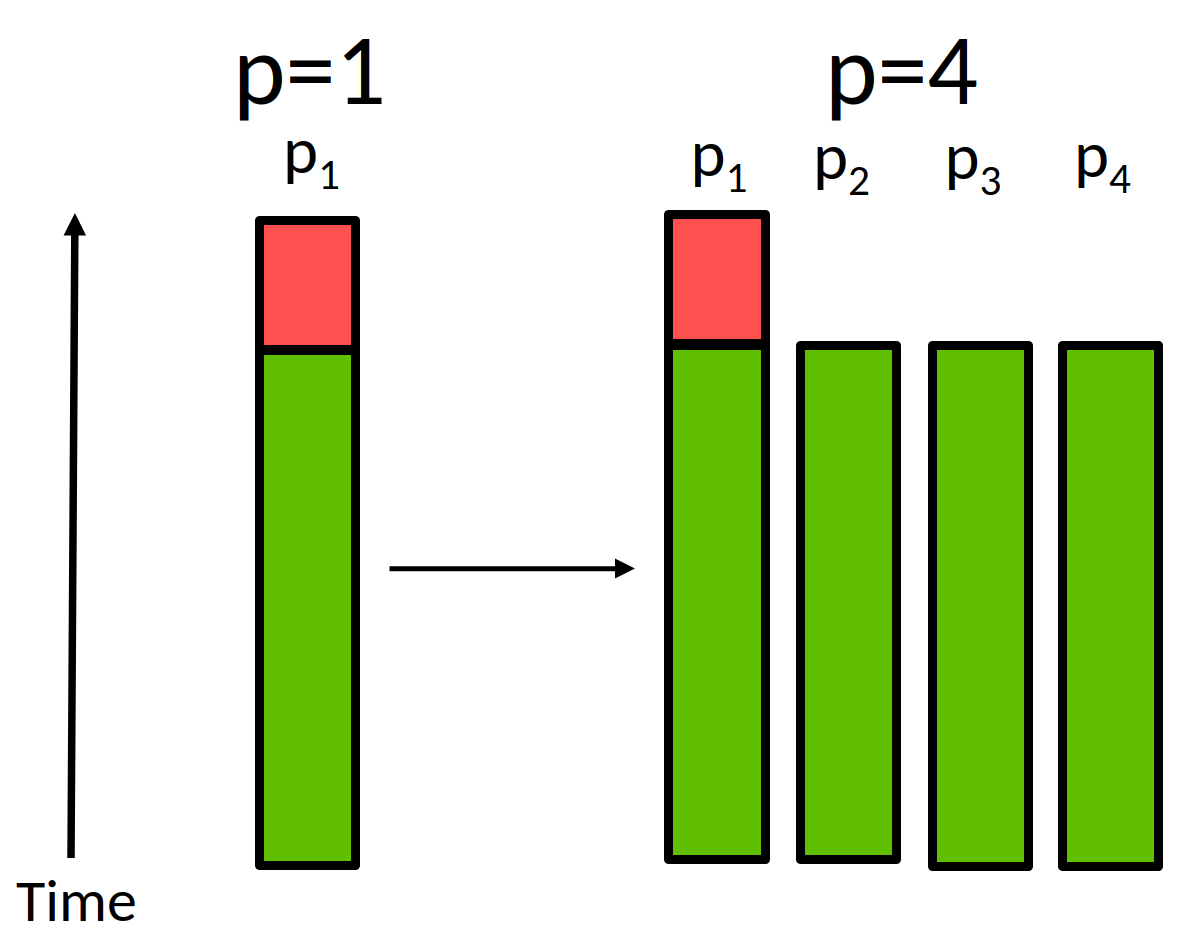
\includegraphics[scale=0.15]{gustafson.png}
    \caption{Red Part is Sequential Work, Green Part is Parallelizable Work.}
\end{figure}

\noindent Note that each processor gets the entire green part to execute. On four processors, more work is done than on one. This was not the case with Amdahl's law.\\[3mm]
Let $W$ denote the work done in a fixed time interval. We can write
\begin{equation*}
    W = \mathbf{f} * W + (1 - \mathbf{f}) * W
\end{equation*}
Where \textbf{f} is the sequential fraction of $T_{1}$. As we increase the number of processors at our disposal, we multiply the parallel fraction of our program. The serial fraction remains the same. Letting $W_P$ be the work done with $P$ processors at our disposal, we get
\begin{equation*}
    W_P = \mathbf{f} * W + P * (1 - \mathbf{f}) * W
\end{equation*}
In the figure, we can see this as the parallel work (green part) is $(1-\mathbf{f}) * W$ and each of the \textbf{P} processors executes this green part. One processor additionally has to execute the sequential work (red part), which is $\mathbf{f}*W$.\\
We can now follow \textit{Gustafson's law}.
\begin{theorem}
    Let $\mathbf{f}$ denote the non-parallelizable, serial fraction of the total work done in the program and P the number of processors at our disposal. Then, we get
    \begin{align*}
        S_P &= \mathbf{f} + P(1-f)\\
            &= P - \mathbf{f}(P-1)
    \end{align*}
\end{theorem}
We can see this result directly from the figure. Let us normalize the runtime (on \textbf{P} processors) to one. We simply ask ourselves how long it takes a single processor to execute all the work that the \textbf{P} processors do. And this work is given by the equation $W_P = \mathbf{f} * W + P * (1 - \mathbf{f}) * W$. So, a single processor needs to execute the parallel part \textbf{P} times and the sequential part once. We can visualize the speedup now as all the green parts plus one red part stacked on top of each other (runtime on one processor) versus just one red and one green part (runtime on \textbf{P} processors, because all the other green parts are computed in parallel and thus do not add to the runtime).

If we again consider a program where 25\% is non-parallelizable, we get a speedup of 4 already when we increase the number of processors to 5.

It has to be noted that Gustafson's law is only formulated for a certain class of problems where problem size can be scaled when additional computational resources are available. For example Amdahl's law might be better applicable to problems like sorting a fixed set of integers, but Gustafson's law could be used to describe the problem of rendering a 3D-scene as detailed as possible - the level of detail can be increased in the case of 3D-rendering, but there is no such thing as sorting a set of integers in a more exact way.

\end{document}
